% Created 2024-04-09 Tue 14:23
% Intended LaTeX compiler: pdflatex
\documentclass[11pt]{article}
\usepackage[utf8]{inputenc}
\usepackage[T1]{fontenc}
\usepackage{graphicx}
\usepackage{longtable}
\usepackage{wrapfig}
\usepackage{rotating}
\usepackage[normalem]{ulem}
\usepackage{amsmath}
\usepackage{amssymb}
\usepackage{capt-of}
\usepackage{hyperref}
\usepackage{listings}
\usepackage{color}
\usepackage{amsmath}
\usepackage{array}
\usepackage[T1]{fontenc}
\usepackage{natbib}
\author{Anders Munch}
\date{\today}
\title{}
\begin{document}

\tableofcontents

Remember to exceture (C-c C-c) the following line:


\section{Packages and setup}
\label{sec:org03ea286}
\begin{verbatim}
riskRegression version 2023.12.21

 randomForestSRC 3.2.3 
 
 Type rfsrc.news() to see new features, changes, and bug fixes. 
 

data.table 1.14.10 using 4 threads (see ?getDTthreads).  Latest news: r-datatable.com
\end{verbatim}


\section{sandbox}
\label{sec:org19b5a97}
\#+RESULTS[(2024-04-03 12:10:39) fee665afcd6283305bb47ea7788468cc4d229ad4]:

\section{CV}
\label{sec:orgc34b6a9}

\begin{center}
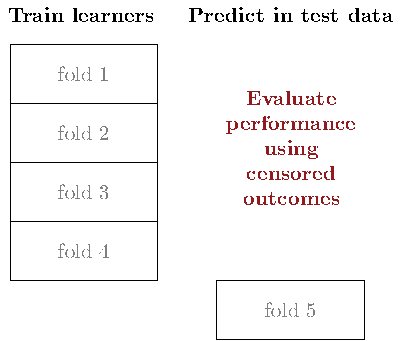
\includegraphics[width=.9\linewidth]{cv-viz.pdf}
\end{center}

\section{Motivation}
\label{sec:orge704139}


\begin{center}
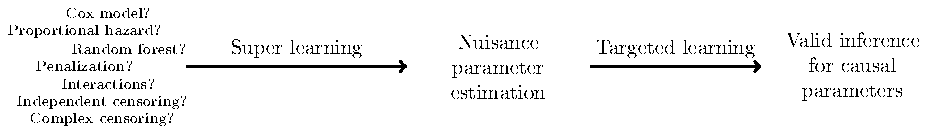
\includegraphics[width=.9\linewidth]{motivation.pdf}
\end{center}

\section{Hold-out sample problem}
\label{sec:orgeb1f1f9}
\begin{center}
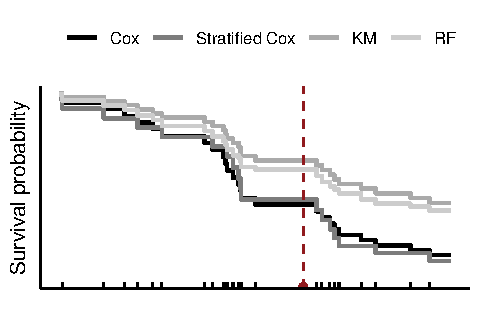
\includegraphics[width=.9\linewidth]{sl-hold-out-sample.pdf}
\end{center}



\section{IPCW circel}
\label{sec:org05a74bf}

\begin{center}
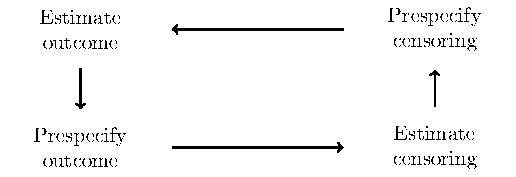
\includegraphics[width=.9\linewidth]{ipcw-circle.pdf}
\end{center}

\begin{center}
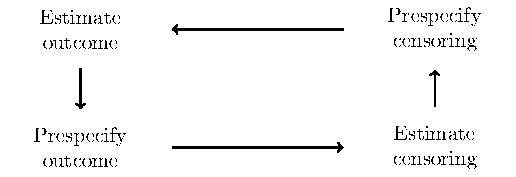
\includegraphics[width=.9\linewidth]{ipcw-circle.pdf}
\end{center}

\section{Censoring and multi-state system}
\label{sec:org331a06f}

\begin{center}
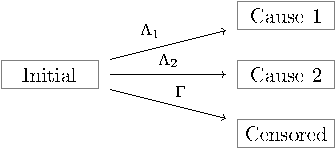
\includegraphics[width=.9\linewidth]{comp-risk-observed-w-text.pdf}
\end{center}

\begin{center}
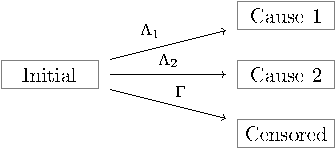
\includegraphics[width=.9\linewidth]{comp-risk-observed-w-text.pdf}
\end{center}


\begin{center}
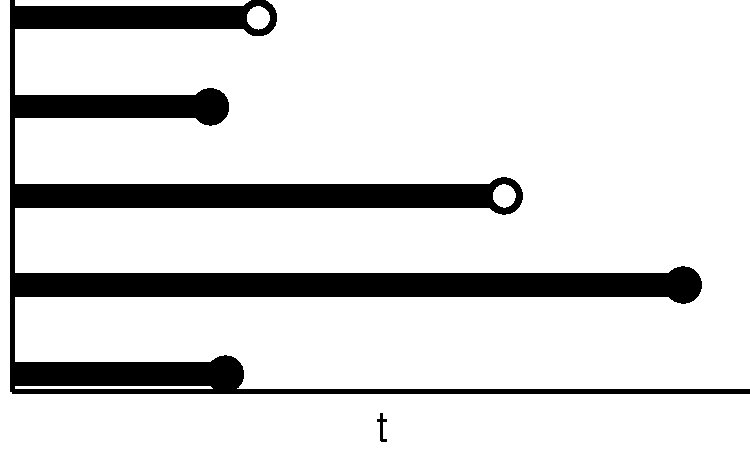
\includegraphics[width=.9\linewidth]{./multi-state-data-1.pdf}
\end{center}

\begin{center}
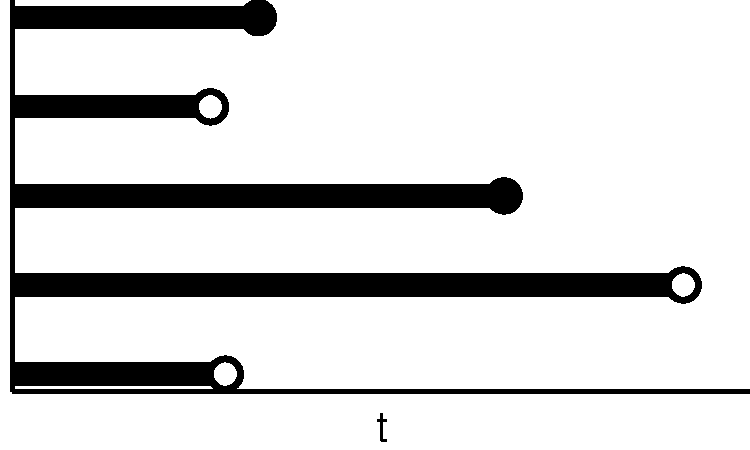
\includegraphics[width=.9\linewidth]{./multi-state-data-2.pdf}
\end{center}

\begin{center}
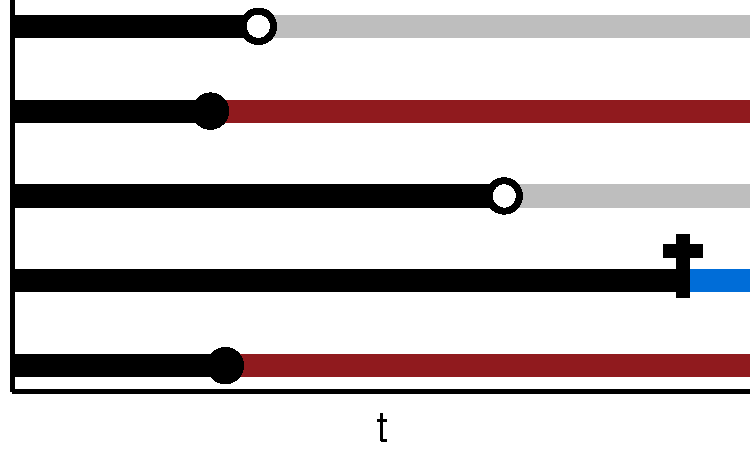
\includegraphics[width=.9\linewidth]{./multi-state-data-3.pdf}
\end{center}

\section{Simulation study}
\label{sec:org4dbd4e5}

\begin{verbatim}
     n_obs    sim_set  type            SL time type.1       IPA           se
  1:   300   original  cens        survSL    6   cens 0.6978450 0.0008305614
  2:   300   original  cens State learner    6   cens 0.6989384 0.0008192387
  3:   300   original  cens        Oracle    6   cens 0.6992857 0.0008149009
  4:   300   original event        survSL    6  event 0.3488385 0.0019823097
  5:   300   original event State learner    6  event 0.3468667 0.0019972122
 ---                                                                        
380:  2400 indep_cens event        survSL   36  event 0.1922440 0.0003727166
381:  2400 indep_cens event State learner   36  event 0.2005905 0.0002755740
382:  2400 indep_cens event      IPCW(KM)   36  event 0.2005905 0.0002755740
383:  2400 indep_cens event     IPCW(Cox)   36  event 0.2005905 0.0002755740
384:  2400 indep_cens event        Oracle   36  event 0.2005905 0.0002755740
     n_obs               sim_set  type            SL time type.1       IPA           se
  1:   300   Dependent censoring  cens        survSL    6   cens 0.6978450 0.0008305614
  2:   300   Dependent censoring  cens State learner    6   cens 0.6989384 0.0008192387
  3:   300   Dependent censoring  cens        Oracle    6   cens 0.6992857 0.0008149009
  4:   300   Dependent censoring event        survSL    6  event 0.3488385 0.0019823097
  5:   300   Dependent censoring event State learner    6  event 0.3468667 0.0019972122
 ---                                                                                   
380:  2400 Independent censoring event        survSL   36  event 0.1922440 0.0003727166
381:  2400 Independent censoring event State learner   36  event 0.2005905 0.0002755740
382:  2400 Independent censoring event      IPCW(KM)   36  event 0.2005905 0.0002755740
383:  2400 Independent censoring event     IPCW(Cox)   36  event 0.2005905 0.0002755740
384:  2400 Independent censoring event        Oracle   36  event 0.2005905 0.0002755740
\end{verbatim}

\#	 aes(x = n\textsubscript{obs}, y = IPA, col = SL)) +

\#		  aes(ymin = IPA-1.96*se, ymax = IPA+1.96*se),
\#		  width = .1,
\#		  alpha = .5,
\#		  size = 1) + 

\begin{center}
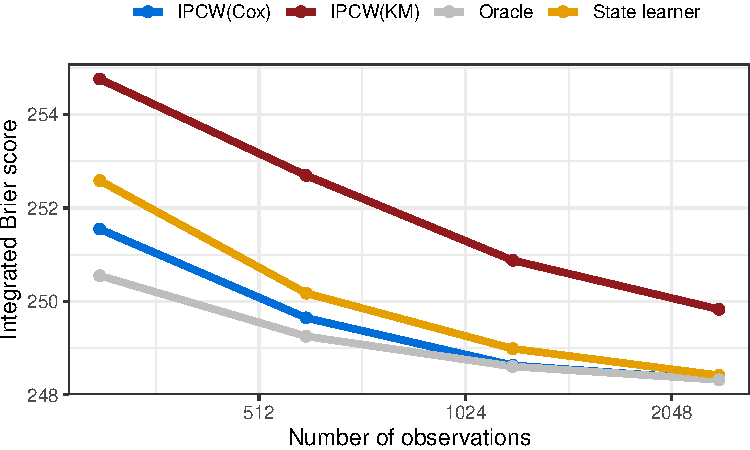
\includegraphics[width=.9\linewidth]{experiment-fig-sl-ipcw.pdf}
\end{center}

DRop this

\section{Illustration zelefsky data}
\label{sec:orgbf55166}

\begin{center}
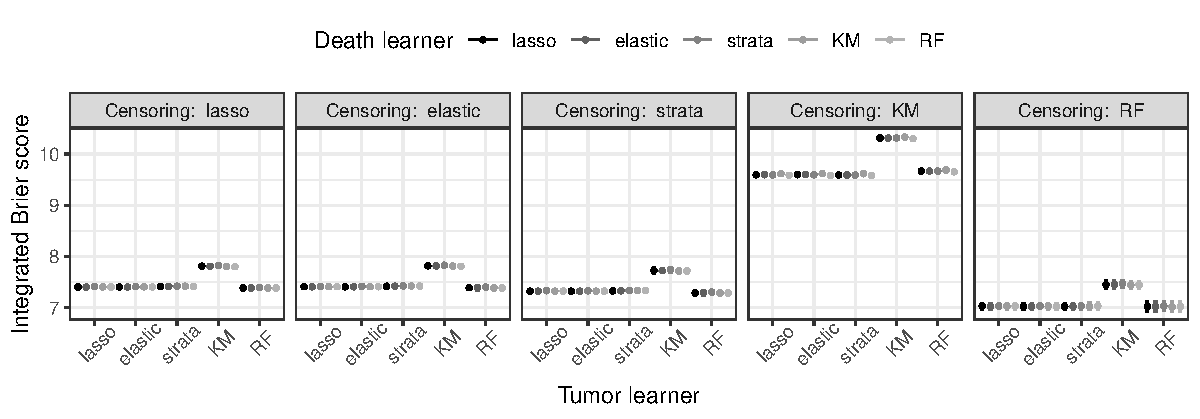
\includegraphics[width=.9\linewidth]{zelefski-real-data.pdf}
\end{center}


\begin{center}
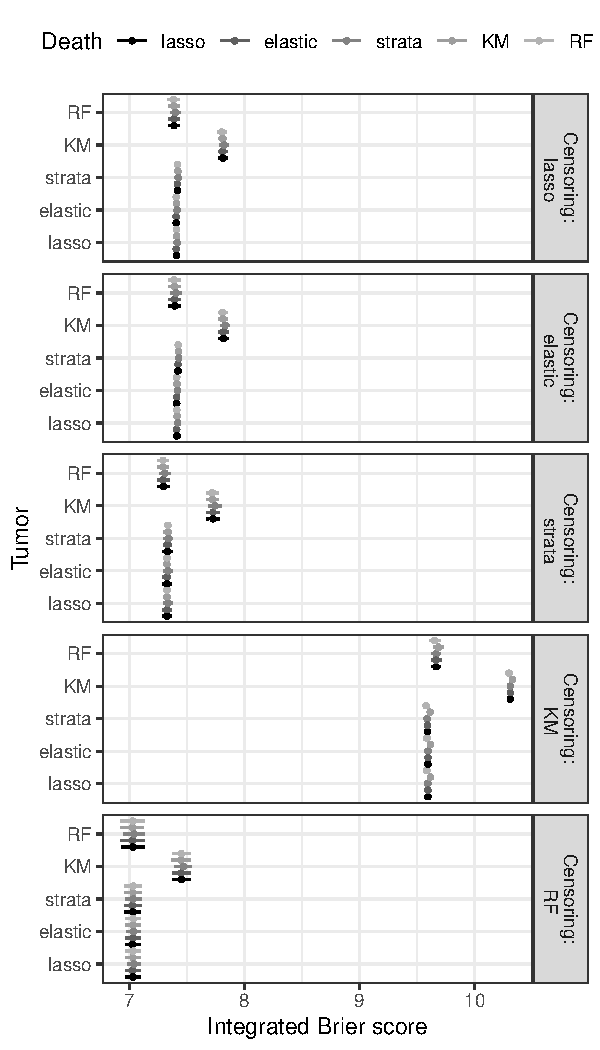
\includegraphics[width=.9\linewidth]{zelefski-real-data-flip.pdf}
\end{center}

\begin{verbatim}
     cause1  cause2 censor      loss
  1:     RF      KM     RF  7.022057
  2: strata elastic     RF  7.025097
  3:     RF elastic     RF  7.025267
  4:     RF      RF     RF  7.025504
  5: strata   lasso     RF  7.025648
 ---                                
121:     KM      RF     KM 10.299304
122:     KM   lasso     KM 10.310004
123:     KM elastic     KM 10.310062
124:     KM  strata     KM 10.310763
125:     KM      KM     KM 10.328653
\end{verbatim}


\#	plot\textsubscript{data}[,cause:=factor(cause,levels=c("cause1","cause2"),labels=c("Tumor recurrence","Death"))]
\#	ggplot(plot\textsubscript{data}, aes(x = time, y = est)) +
\#	  geom\textsubscript{errorbar}(aes(ymin = lower, ymax = upper), width = 1) + 
\#	  geom\textsubscript{point}() +
\#	  geom\textsubscript{hline}(yintercept = 0, linetype = 2) +
\#	  theme\textsubscript{bw}() +
\#	  facet\textsubscript{wrap}( \textasciitilde{} cause) +
\#	  xlab("Months after baseline") + ylab("ATE of hormone therapy") +
\#	  scale\textsubscript{x}\textsubscript{continuous}(breaks = seq(6,36,12)) +
\#	  scale\textsubscript{y}\textsubscript{continuous}(labels = scales::percent)


\begin{center}
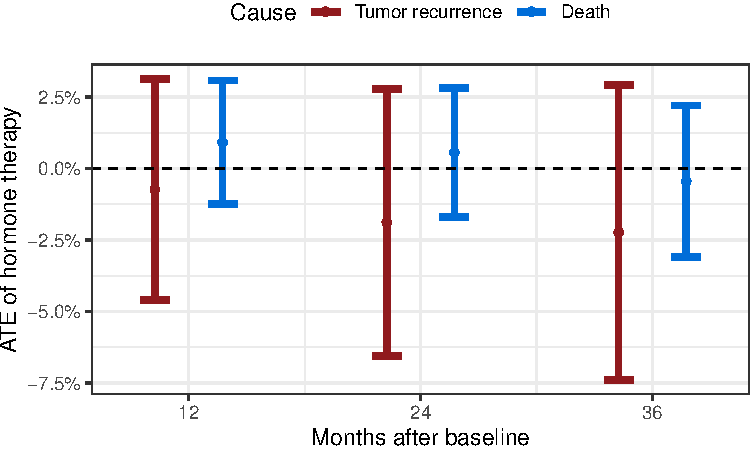
\includegraphics[width=.9\linewidth]{zelefsky-data-target-par.pdf}
\end{center}
\end{document}